%%%%%%%%%%%%%% 27/02/2020 %%%%%%%%%%%%%%%% 
\subsection*{\textbf{27/02/2020}}
\subsubsection*{Days aims}
\begin{itemize}
    \item Finalize cuts to be made on $Z \rightarrow ee$ and $Z \rightarrow \mu\mu$
\end{itemize}

\subsubsection*{Day Summary}
\begin{itemize}
    \item Plotted total ptcone30
    \item Plotted total etcone20 
    \item Plotted PT of single leptons 
    \item Plotted the invaraint mass of ee and mumu pair 

    \item Cut on pT
    \subitem $Z \rightarrow ee$ = $36 GeV < p_T$
    \subitem $Z \rightarrow \mu\mu$ = $34 GeV < p_T$
    
    \item Cut on ptcone30 
    \subitem $Z \rightarrow ee$ = $ ptcone < 5.8 GeV$
    \subitem $Z \rightarrow \mu\mu$ = $ ptcone < 6.5 GeV$
    
    \item Cut on etcone20 
    \subitem $Z \rightarrow ee$ = $ -2 GeV < etcone < 6 GeV$
    \subitem $Z \rightarrow \mu\mu$ = $ -1.6 GeV < etcone < 5.25 GeV$
    
    \item Cut on invariant mass  
    \subitem $Z \rightarrow ee$ = $70 GeV < m_{ll} < 150 GeV$
    \subitem $Z \rightarrow \mu\mu$ = $60 GeV < m_{ll} < 150 GeV$
    
    \item Started to calculate cross sections for Z
\end{itemize}

%%%%%%%%%%%%% 9:00 %%%%%%%%%%%%%
\subsubsection*{09:00 - Lead BG}
Start by Plotting each variable, with and without a specific cut, and calculating the cross section for each.
\\
Make new notebook - \textit{DoubleHist} - to compare ATLAS data and a single MC data 

%%%%%%%%%%%%% 9:36 %%%%%%%%%%%%%
\subsubsection*{09:36}
Plot the ptcone30 for ee and $\mu\mu$ on sperate graphs on Fig.\ref{fig:All-stack-Zll-fast_(basic-cuts_2lep=ll_opp-c)_27-02-2021_09-50} with the cuts
\begin{lstlisting}
    # e=11, mu=13
    lepCut ="(" + "(lep_charge[0] != lep_charge[1]) && (lep_type[0]== 11 && lep_type[1] == 11) && lep_n==2" + ")"
    
    t.SetAlias("inv_mass_Zll","sqrt(2*lep_pt[0]*lep_pt[1]*(cosh(lep_eta[0]-lep_eta[1])-cos(lep_phi[0]-lep_phi[1])))")
    t.Draw("lep_ptcone30[0]+lep_ptcone30[1] >> h_lep_ptcone30(300,0,12e3)", weighting + "*" + lepCut)
\end{lstlisting}

\begin{figure}[h!]
    \centering
    \begin{minipage}{0.5\textwidth}
        \centering
        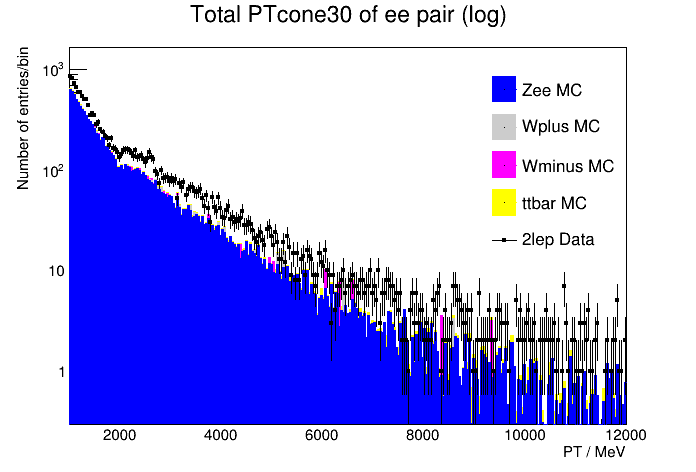
\includegraphics[width=\linewidth]{plots/27-02-2021/All-stack-Zee-fast_(basic-cuts_2lep=ee_opp-c)_27-02-2021_09-50.png}
        (A)
    \end{minipage}\hfill
    \begin{minipage}{0.5\textwidth}
        \centering
        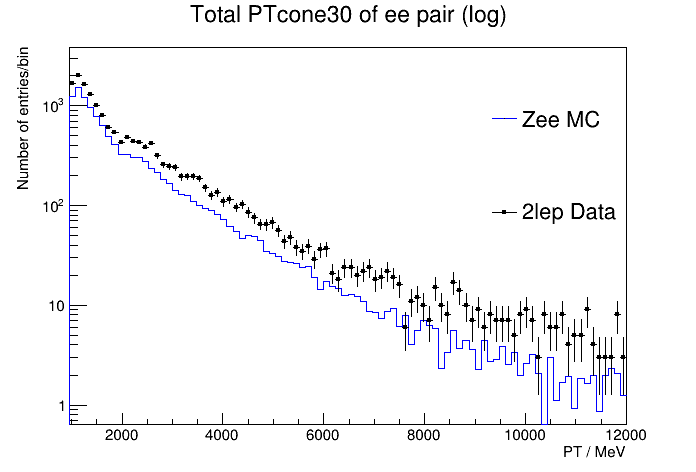
\includegraphics[width=\linewidth]{plots/27-02-2021/2-Stack-Zee-2lep-fast_(basic-ee_opp-c)_27-02-21_10-00).png}
        (B)
    \end{minipage}
    \caption{(A) Total ptcone30 on a log-y graph for ee pair with simulated background (B) Total ptcone30 on a log-y graph for ee pair with simulated background. (only Basic) Cuts: lep-n=2, same type, opposite charge}
    \label{fig:All-stack-Zll-fast_(basic-cuts_2lep=ll_opp-c)_27-02-2021_09-50}
\end{figure}


From \ref{} the ATLAS data follows the MC. data well for 


\subsubsection*{10:05}
Apply the Invariant mass cut the the ptcone log plot to see if that changes for ee


\begin{figure}[h!]
    \centering
    \begin{minipage}{0.5\textwidth}
        \centering
        \includegraphics[width=\linewidth]{plots/27-02-2021/}
        (A)
    \end{minipage}\hfill
    \begin{minipage}{0.5\textwidth}
        \centering
        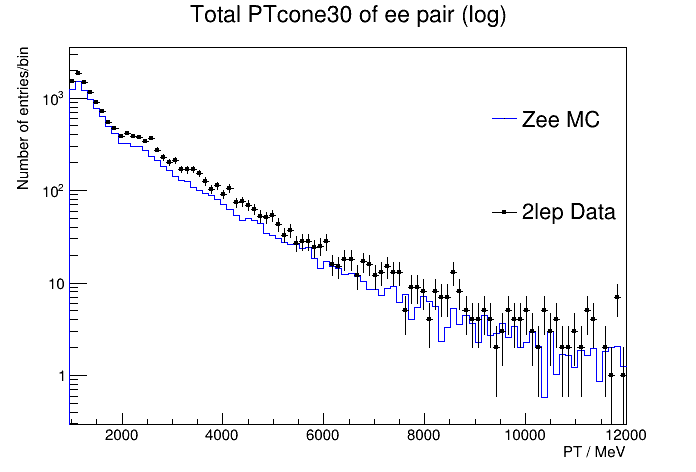
\includegraphics[width=\linewidth]{plots/27-02-2021/2-Stack-Zee-2lep-fast_(basic-and_invarmass-lower=60GeV)_27-02-21_10-10).png}
        (B)
    \end{minipage}
    \caption{(A)  (B) Total ptcone30 of ee pair for ATLAS and Zmumu MC. Cuts: invar-mass-lower=60GeV, pair of mu with opposite charge.}
    \label{}
\end{figure}

%%%%%%%%%%%%% 10:17 %%%%%%%%%%%%%
\subsubsection*{10:17}
Plot the total ptone30 for mumu on a log-y plot
with the cuts used in Fig.\ref{fig:stack-Zmumu-fast_(invar-mass-lower=60GeV)_27-02-21_10-19} to include a lower bound on the invariant mass:
\begin{lstlisting}
lepCut ="(" + "(lep_charge[0] != lep_charge[1]) && (lep_type[0]== 13 && lep_type[1] == 13) && lep_n==2 " + ")"
    
t.SetAlias("inv_mass_Zll","sqrt(2*lep_pt[0]*lep_pt[1]*(cosh(lep_eta[0]-lep_eta[1])-cos(lep_phi[0]-lep_phi[1])))")

t.Draw("lep_ptcone30[0]+lep_ptcone30[1] >> h_lep_ptcone30(100,0,12e3)", weighting + "*" + lepCut)
\end{lstlisting}
% invar mas 
\begin{figure}[h!]
    \centering
    \begin{minipage}{0.5\textwidth}
        \centering
        \includegraphics[width=\linewidth]{plots/27-02-2021/}
        (A)
    \end{minipage}\hfill
    \begin{minipage}{0.5\textwidth}
        \centering
        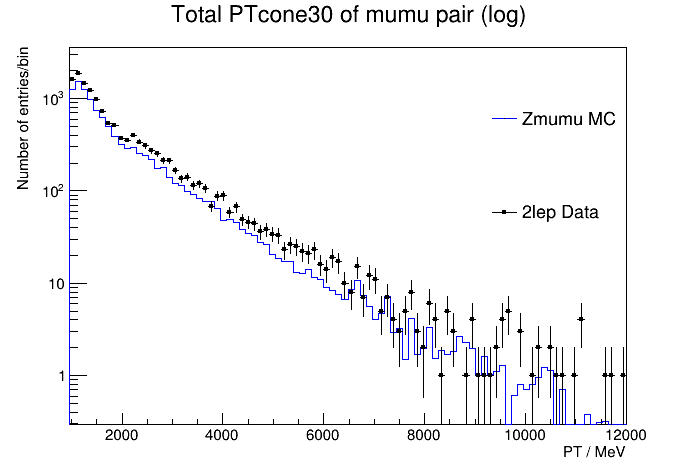
\includegraphics[width=\linewidth]{plots/27-02-2021/2-stack-Zmumu-fast_(invar-mass-lower=60GeV)_27-02-21_10-19.png}
        (B)
    \end{minipage}
    \caption{(A)  (B) ptcone30 of Z -> mumu for the ATLAS and Zmumu MC data. Cuts: invar-mass-lower=60GeV, with basic cuts of mu pair with opposite charge.}
    \label{fig:stack-Zmumu-fast_(invar-mass-lower=60GeV)_27-02-21_10-19}
\end{figure}

%%%%%%%%%%%%% 10:27 %%%%%%%%%%%%%
\subsubsection*{10:27}
Plot total ptcone30 for mu pair without invar-mass-lower=60GeV cut.
\\
Cuts using for Fig.\ref{fig:stack-Zmumu-fast_(basics_mu-pair_opp-c)_27-02-21_10-27}
\begin{lstlisting}
lepCut ="(" + "(lep_charge[0] != lep_charge[1]) && (lep_type[0]== 13 && lep_type[1] == 13) && lep_n==2 " + ")"
    
t.SetAlias("inv_mass_Zll","sqrt(2*lep_pt[0]*lep_pt[1]*(cosh(lep_eta[0]-lep_eta[1])-cos(lep_phi[0]-lep_phi[1])))")

t.Draw("lep_ptcone30[0]+lep_ptcone30[1] >> h_lep_ptcone30(100,0,12e3)", weighting + "*" + lepCut)
\end{lstlisting}

\begin{figure}[h!]
    \centering
    \begin{minipage}{0.5\textwidth}
        \centering
        \includegraphics[width=\linewidth]{plots/27-02-2021/}
        (A)
    \end{minipage}\hfill
    \begin{minipage}{0.5\textwidth}
        \centering
        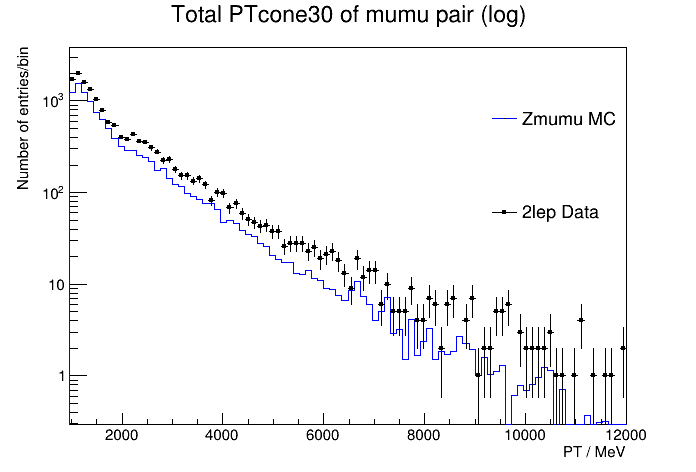
\includegraphics[width=\linewidth]{plots/27-02-2021/2-stack-Zmumu-fast_(basics_mu-pair_opp-c)_27-02-21_10-27.png}
        (B)
    \end{minipage}
    \caption{(A)  (B) Total ptcone30 of $Z -> \mu\mu$ for the ATLAS and Zmumu MC data. With basic cuts of mu pair with opposite charge.}
    \label{fig:stack-Zmumu-fast_(basics_mu-pair_opp-c)_27-02-21_10-27}
\end{figure}


%%%%%%%%%%%%% 10:30 %%%%%%%%%%%%%
\subsubsection*{10:30}
Plotting the total etcone20 of ee pair with only basic cuts on log-y plot.
\\
Cuts used in Fig.\ref{}
\begin{lstlisting}
lepCut ="(" + "(lep_charge[0] != lep_charge[1]) && (lep_type[0]== 11 && lep_type[1] == 11) && lep_n==2" + ")"    
    
t.SetAlias("inv_mass_Zll","sqrt(2*lep_pt[0]*lep_pt[1]*(cosh(lep_eta[0]-lep_eta[1])-cos(lep_phi[0]-lep_phi[1])))")

t.Draw("(lep_etcone20[0] + lep_etcone20[1]) >> h_lep_etcone20(100,-7e3,14e3)", weighting + "*" + lepCut)
\end{lstlisting}
\begin{figure}[h!]
    \centering
    \begin{minipage}{0.5\textwidth}
        \centering
        \includegraphics[width=\linewidth]{plots/27-02-2021/}
        (A)
    \end{minipage}\hfill
    \begin{minipage}{0.5\textwidth}
        \centering
        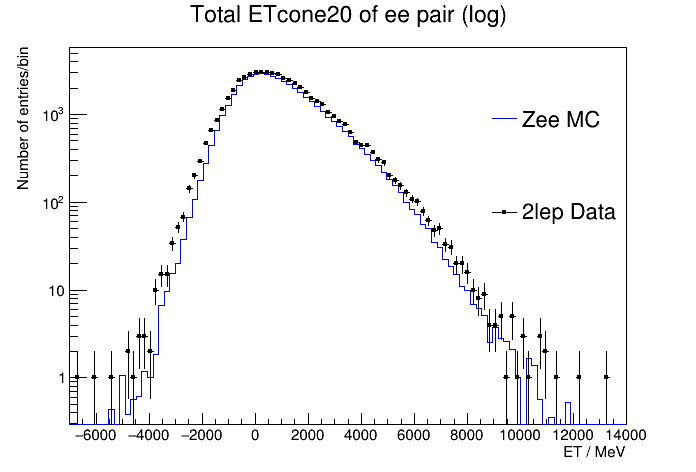
\includegraphics[width=\linewidth]{plots/27-02-2021/2-Stack-Zee-fast_total-etcone_(basic-cuts_ee-pair-opp-c)_27-02-21_10-35.png}
        (B)
    \end{minipage}
    \caption{(A)  (B) Total etcone20 of ee pair for ATLAS and Zee MC. Cuts: (only basic) ee pair with opposite charge.}
    \label{}
\end{figure}

%%%%%%%%%%%%% 10:39 %%%%%%%%%%%%%
\subsubsection*{10:39}
Plotting the single etcone20 of one of the particle of the ee pair with only basic cuts on log-y plot.
\\
Cuts used in Fig.\ref{fig:2-Stack-Zee-fast_etcone[0]_(basic-ee_opp-c)_27-02-21_10-39}
\begin{lstlisting}
lepCut ="(" + "(lep_charge[0] != lep_charge[1]) && (lep_type[0]== 11 && lep_type[1] == 11) && lep_n==2" + ")"    
    
t.SetAlias("inv_mass_Zll","sqrt(2*lep_pt[0]*lep_pt[1]*(cosh(lep_eta[0]-lep_eta[1])-cos(lep_phi[0]-lep_phi[1])))")

t.Draw("lep_etcone20[0] >> h_lep_etcone20(100,-7e3,14e3)", weighting + "*" + lepCut)
\end{lstlisting}

\begin{figure}[h!]
    \centering
    \begin{minipage}{0.5\textwidth}
        \centering
        \includegraphics[width=\linewidth]{plots/27-02-2021/}
        (A)
    \end{minipage}\hfill
    \begin{minipage}{0.5\textwidth}
        \centering
        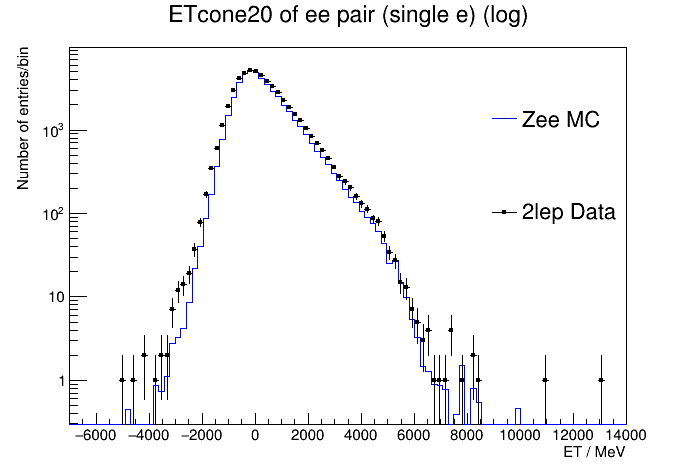
\includegraphics[width=\linewidth]{plots/27-02-2021/2-Stack-Zee-fast_etcone[0]_(basic-ee_opp-c)_27-02-21_10-39.png}
        (B)
    \end{minipage}
    \caption{(A)  (B) Single etcone20 of a single particle for ee pair.  Cuts: (only basic) ee pair with opposite charge}
    \label{fig:2-Stack-Zee-fast_etcone[0]_(basic-ee_opp-c)_27-02-21_10-39}
\end{figure}

%%%%%%%%%%%%% 10:50 %%%%%%%%%%%%% - etcone20 (single muon) (log-y)
\subsubsection*{10:50 - etcone20 of single muon (log-y)}
Potting the etcone20 of a single muon of a mumu pair on a log-y plot using only the basic cuts (mumu pair with opposite charge).
\\
The cuts used in Fig.\ref{fig:Stack-Zmumu-fast_single-etcone_(basic-cuts_2mumu-pair-opp-c)_27-02-21_10-50}
\begin{lstlisting}
lepCut ="(" + "(lep_charge[0] != lep_charge[1]) && (lep_type[0]== 13 && lep_type[1] == 13) && lep_n==2" + ")"    
    
t.SetAlias("inv_mass_Zll","sqrt(2*lep_pt[0]*lep_pt[1]*(cosh(lep_eta[0]-lep_eta[1])-cos(lep_phi[0]-lep_phi[1])))")

t.Draw("lep_etcone20[0] >> h_lep_etcone20(100,-7e3,14e3)", weighting + "*" + lepCut)
\end{lstlisting}

\begin{figure}[h!]
    \centering
    \begin{minipage}{0.5\textwidth}
        \centering
        \includegraphics[width=\linewidth]{plots/27-02-2021/}
        (A)
    \end{minipage}\hfill
    \begin{minipage}{0.5\textwidth}
        \centering
        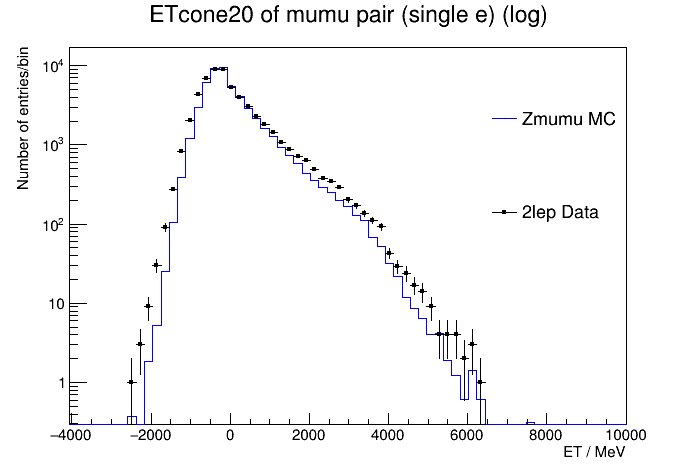
\includegraphics[width=\linewidth]{plots/27-02-2021/2-stack-Zmumu-fast_single-etcone_(basic-cuts_2mumu-pair-opp-c)_27-02-21_10-50.png}
        (B)
    \end{minipage}
    \caption{(A)  (B) etcone20 of single muon for both ATLAS and Zmumu.  Cuts: (basic only) }
    \label{fig:Stack-Zmumu-fast_single-etcone_(basic-cuts_2mumu-pair-opp-c)_27-02-21_10-50}
\end{figure}

%%%%%%%%%%%%% 10:57 %%%%%%%%%%%%% - Difference in etcone (log-y)
\subsubsection*{10:57 - Difference in etcone}
Plotting the difference in etcone20 for mumu with only the basic cuts being used in Fig.\ref{fig:Stack-Zmumu-fast_etcone-difference_log-y_(basic-cuts_2lep=mumu_opp-c)_27-02-21_10-57}:
\begin{lstlisting}
lepCut ="(" + "(lep_charge[0] != lep_charge[1]) && (lep_type[0]== 13 && lep_type[1] == 13) && lep_n==2" + ")"    
    
t.SetAlias("inv_mass_Zll","sqrt(2*lep_pt[0]*lep_pt[1]*(cosh(lep_eta[0]-lep_eta[1])-cos(lep_phi[0]-lep_phi[1])))")
    
t.Draw("abs(lep_etcone20[0]-lep_etcone20[1]) >> h_lep_etcone20(100,-7e3,14e3)", weighting + "*" + lepCut)
\end{lstlisting}

\begin{figure}[h!]
    \centering
    \begin{minipage}{0.5\textwidth}
        \centering
        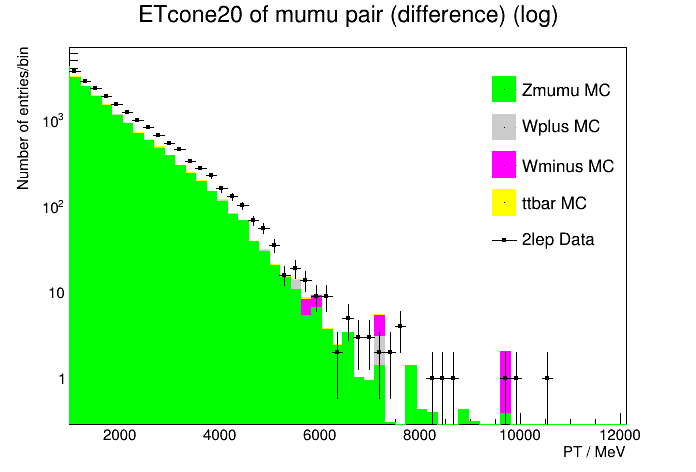
\includegraphics[width=\linewidth]{plots/27-02-2021/All-Stack-Zmumu-fast_etcone-difference_log-y_(basic-cuts_2lep=mumu_opp-c)_27-02-21_10-57.png}
        (A)
    \end{minipage}\hfill
    \begin{minipage}{0.5\textwidth}
        \centering
        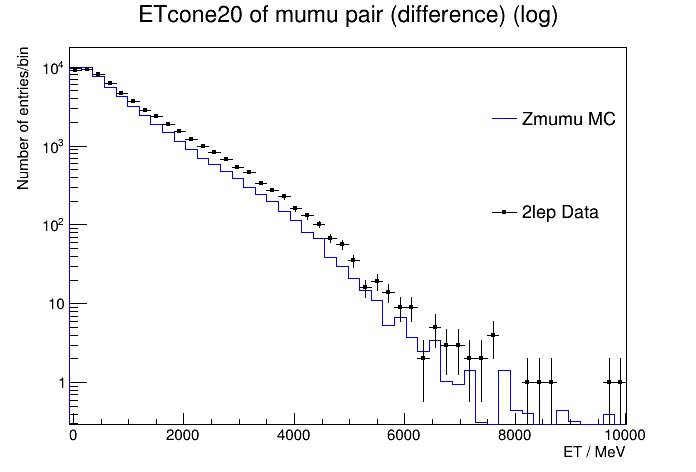
\includegraphics[width=\linewidth]{plots/27-02-2021/2-Stack-Zmumu-fast_etcone-difference_log-y_(basic-cuts_2lep=mumu_opp-c)_27-02-21_10-57.png}
        (B)
    \end{minipage}
    \caption{(A) The absolute difference in etcone20 for ATLAS, MC and MC background. (B) The absolute difference in etcone20 for $Z \rightarrow \mu\mu$ using both ATLAS and MC data.  Cuts: (only basic) mumu pair with opposite charge}
    \label{fig:Stack-Zmumu-fast_etcone-difference_log-y_(basic-cuts_2lep=mumu_opp-c)_27-02-21_10-57}
\end{figure}


%%%%%%%%%%%%% 11:05 %%%%%%%%%%%%% - Difference in etcone
\subsubsection*{11:05 - Difference in etcone}
Plotting the absolute difference in etcone20 for mumu pair of opposite charge.
\\
Cuts used in Fig.\ref{fig:Stack-Zmumu-fast_etcone-difference_(basic-cuts_2lep=mumu_opp-c)_27-02-21_11-05}:
\begin{lstlisting}
lepCut ="(" + "(lep_charge[0] != lep_charge[1]) && (lep_type[0]== 13 && lep_type[1] == 13) && lep_n==2" + ")"    
    
t.SetAlias("inv_mass_Zll","sqrt(2*lep_pt[0]*lep_pt[1]*(cosh(lep_eta[0]-lep_eta[1])-cos(lep_phi[0]-lep_phi[1])))")
   
t.Draw("abs(lep_etcone20[0]-lep_etcone20[1]) >> h_lep_etcone20(100,-7e3,14e3)", weighting + "*" + lepCut)
\end{lstlisting}

\begin{figure}[h!]
    \centering
    \begin{minipage}{0.5\textwidth}
        \centering
        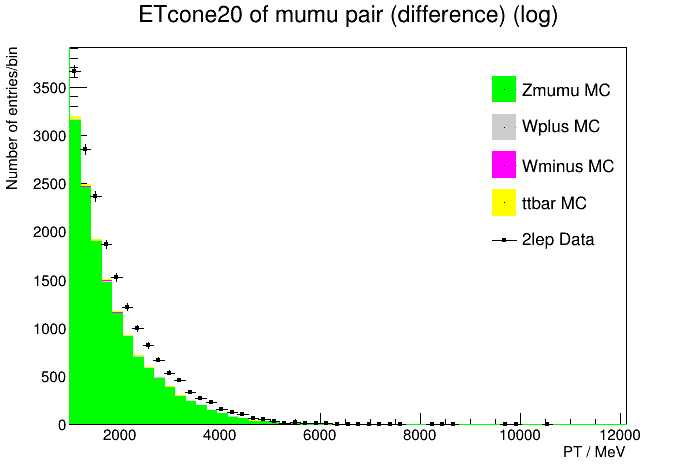
\includegraphics[width=\linewidth]{plots/27-02-2021/All-Stack-Zmumu-fast_etcone-difference_(basic-cuts_2lep=mumu_opp-c)_27-02-21_11-05.png}
        (A)
    \end{minipage}\hfill
    \begin{minipage}{0.5\textwidth}
        \centering
        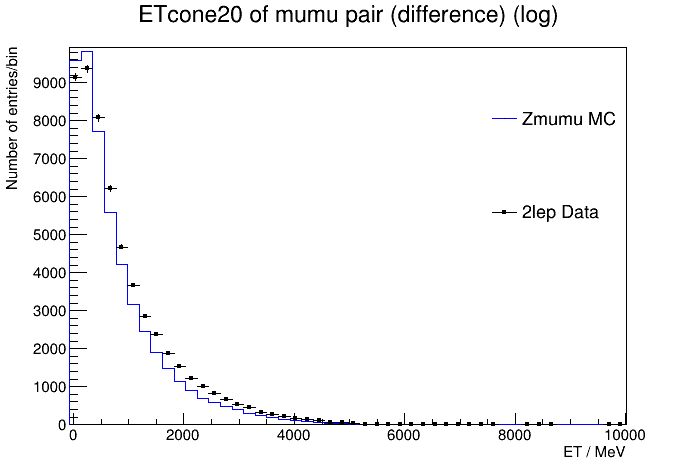
\includegraphics[width=\linewidth]{plots/27-02-2021/2-Stack-Zmumu-fast_etcone-difference_(basic-cuts_2lep=mumu_opp-c)_27-02-21_11-05.png}
        (B)
    \end{minipage}
    \caption{(A) The absolute difference in etcone20 for ATLAS, MC and MC background. (B) The absolute difference in etcone20 for $Z \rightarrow \mu\mu$.  Cuts: (only basic) mumu pair with opposite charge }
    \label{fig:Stack-Zmumu-fast_etcone-difference_(basic-cuts_2lep=mumu_opp-c)_27-02-21_11-05}
\end{figure}



%%%%%%%%%%%%% 11:30 %%%%%%%%%%%%% - ptcone30 for single electron from ee pair (log-y
\subsubsection*{11:30 - ptcone30 for single e from ee pair (log-y)}
PLotting the ptcone30 for a single electron on a log-y plot.
\\
Cuts used in Fig.\ref{fig:stack-Zee-fast_ptcone30-single_log-y_(basics_2lep=ee-opp-c)_27-02-21_11-30}:
\begin{lstlisting}
....
\end{lstlisting}
\begin{figure}[h!]
    \centering
    \begin{minipage}{0.5\textwidth}
        \centering
        \includegraphics[width=\linewidth]{plots/27-02-2021/}
        (A)
    \end{minipage}\hfill
    \begin{minipage}{0.5\textwidth}
        \centering
        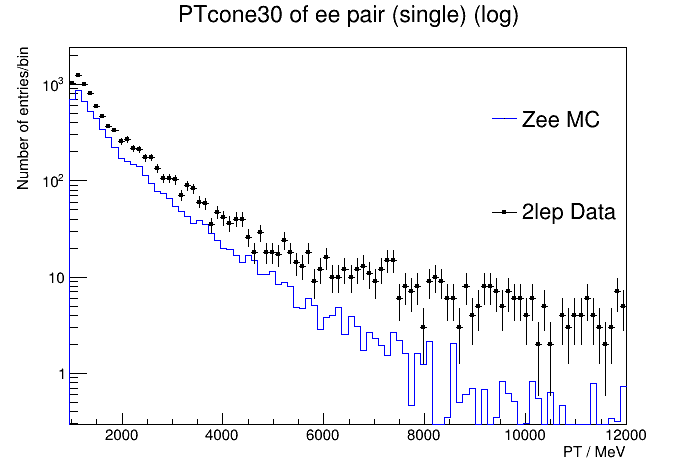
\includegraphics[width=\linewidth]{plots/27-02-2021/2-stack-Zee-fast_ptcone30-single_log-y_(basics_2lep=ee-opp-c)_27-02-21_11-30.png}
        (B)
    \end{minipage}
    \caption{(A)  (B) ptcone30 of single electron from ee pair using the ATLAS and MC Zee data. Cuts: (basic) ee pair with oppsoite charge.}
    \label{fig:stack-Zee-fast_ptcone30-single_log-y_(basics_2lep=ee-opp-c)_27-02-21_11-30}
\end{figure}

%%%%%%%%%%%%% 11:32 %%%%%%%%%%%%% -  ptcone for single muon of mumu pair (log-y
\subsubsection*{11:32 - ptcone30 for single muon in mumu pair (log-y)}
PLotting the ptcone30 for a single muon on a log-y plot.
\\
Cuts using in Fig.\ref{fig:stack-Zmumu-fast_ptcone30-single_log-y_(basics_2lep=mumu-opp-c)_27-02-21_11-30}:
\begin{lstlisting}
....
\end{lstlisting}
\begin{figure}[h!]
    \centering
    \begin{minipage}{0.5\textwidth}
        \centering
        \includegraphics[width=\linewidth]{plots/27-02-2021/}
        (A)
    \end{minipage}\hfill
    \begin{minipage}{0.5\textwidth}
        \centering
        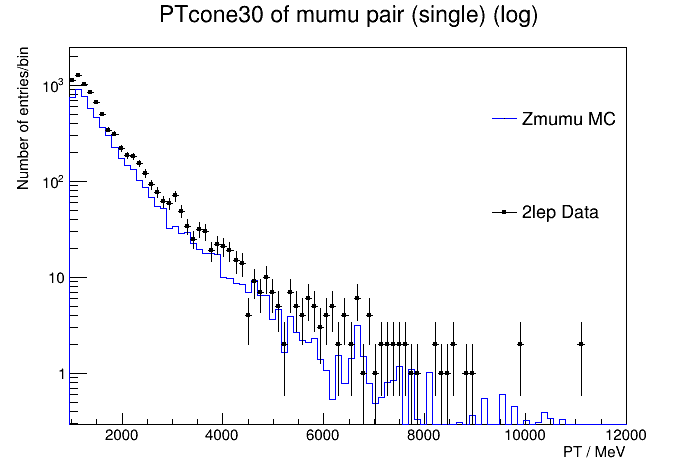
\includegraphics[width=\linewidth]{plots/27-02-2021/2-stack-Zmumu-fast_ptcone30-single_log-y_(basics_2lep=mumu-opp-c)_27-02-21_11-30.png}
        (B)
    \end{minipage}
    \caption{(A)  (B) ptcone30 of single muon from mumu pair using the ATLAS and MC Zmumu data. Cuts: (basic) mumu pair with oppsoite charge. }
    \label{fig:stack-Zmumu-fast_ptcone30-single_log-y_(basics_2lep=mumu-opp-c)_27-02-21_11-30}
\end{figure}

%%%%%%%%%%%%% 11:40 %%%%%%%%%%%%% - PT single e (log-y)
\subsubsection*{11:40 - PT single e (log-y)}
Plotting the transverse momentum for single electron from ee pair with opposite charge on log-y.
\\
Cuts using in Fig.\ref{fig:Stack-Zee-fast_PT-single_log-y_(basic-cuts_2lep=ee_opp-c)_27-02-21_11-40}:
\begin{lstlisting}
lepCut = "(" + "(lep_charge[0] != lep_charge[1]) && (lep_type[0] == 11 && lep_type[1] == 11) && lep_n==2" + ")"

t.SetAlias("inv_mass_Zll","sqrt(2*lep_pt[0]*lep_pt[1]*(cosh(lep_eta[0]-lep_eta[1])-cos(lep_phi[0]-lep_phi[1])))")

t.Draw("lep_pt[0] >> h_lep_pt_total(100, 0,100e3)", weighting + "*" + lepCut)
\end{lstlisting}

\begin{figure}[h!]
    \centering
    \begin{minipage}{0.5\textwidth}
        \centering
        \includegraphics[width=\linewidth]{plots/27-02-2021/}
        (A)
    \end{minipage}\hfill
    \begin{minipage}{0.5\textwidth}
        \centering
        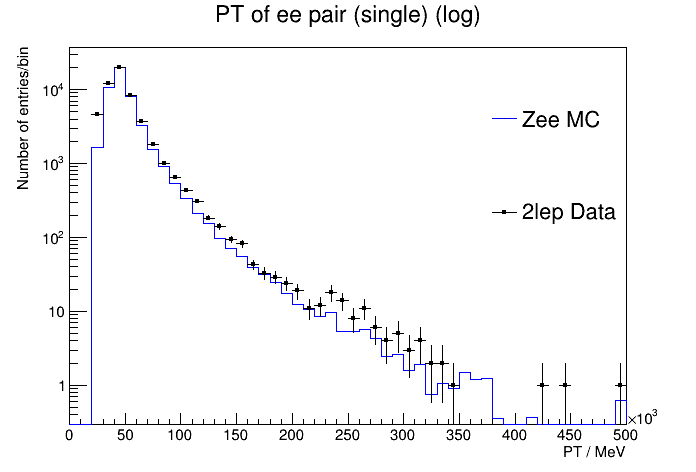
\includegraphics[width=\linewidth]{plots/27-02-2021/2-Stack-Zee-fast_PT-single_log-y_(basic-cuts_2lep=ee_opp-c)_27-02-21_11-40.png}
        (B)
    \end{minipage}
    \caption{(A)  (B) Transverse momentum of a single electron from a ee pair using the ATLAS and MC Zee data.  Cuts: (basic only). ee pair with opposite charge.}
    \label{fig:Stack-Zee-fast_PT-single_log-y_(basic-cuts_2lep=ee_opp-c)_27-02-21_11-40}
\end{figure}


%%%%%%%%%%%%% 11:50 %%%%%%%%%%%%% - PT single mu (log-y)
\subsubsection*{11:50 - PT single mu (log-y)}
Plotting the transverse momentum (PT) of single muon from a mumu pair with opposite charge on a log-y plot.
\\
Cuts used in Fig.\ref{}:
\begin{lstlisting}
lepCut = "(" + "(lep_charge[0] != lep_charge[1]) && (lep_type[0] == 13 && lep_type[1] == 13) && lep_n==2" + ")"

t.SetAlias("inv_mass_Zll","sqrt(2*lep_pt[0]*lep_pt[1]*(cosh(lep_eta[0]-lep_eta[1])-cos(lep_phi[0]-lep_phi[1])))")

t.Draw("lep_pt[0] >> h_lep_pt_total(100, 0,100e3)", weighting + "*" + lepCut)
\end{lstlisting}

% 2-Statck-Zmumu-fast_PT-single_log-y_(basic-cuts_2lep=mumu_opp-c)_27-02-21_11-50.png

\begin{figure}[h!]
    \centering
    \begin{minipage}{0.5\textwidth}
        \centering
        \includegraphics[width=\linewidth]{plots/27-02-2021/}
        (A)
    \end{minipage}\hfill
    \begin{minipage}{0.5\textwidth}
        \centering
        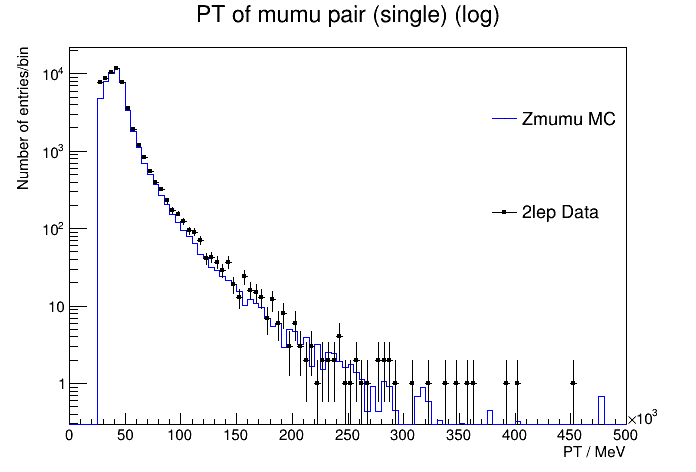
\includegraphics[width=\linewidth]{plots/27-02-2021/2-Statck-Zmumu-fast_PT-single_log-y_(basic-cuts_2lep=mumu_opp-c)_27-02-21_11-50.png}
        (B)
    \end{minipage}
    \caption{(A)  (B) Transverse momentum of a single muon shown for ATLAS and Zmumu MC data.  Cuts: (Basic) mumu pair with opposite charge.}
    \label{}
\end{figure}


%%%%%%%%%%%%% 12:00 %%%%%%%%%%%%% - PT single mu (non-log)
\subsubsection*{12:00 - PT single mu}
% (B) 2-stack-Zmumu-fast_PT-single_(basic_2lep=mumu-opp-c)_27-02-21_12-00.png
Plotting the transverse momentum of single muon of mumu pair of opposite charge on a log-y plot.
\\
Cuts used in Fig.\ref{fig:2-stack-Zmumu-fast_PT-single_(basic_2lep=mumu-opp-c)_27-02-21_12-00}:
\begin{lstlisting}
lepCut = "(" + "(lep_charge[0] != lep_charge[1]) && (lep_type[0] == 11 && lep_type[1] == 11) && lep_n==2" + ")"

t.SetAlias("inv_mass_Zll","sqrt(2*lep_pt[0]*lep_pt[1]*(cosh(lep_eta[0]-lep_eta[1])-cos(lep_phi[0]-lep_phi[1])))")

t.Draw("lep_pt[0] >> h_lep_pt_total(100, 0,100e3)", weighting + "*" + lepCut)
\end{lstlisting}

\begin{figure}[h!]
    \centering
    \begin{minipage}{0.5\textwidth}
        \centering
        \includegraphics[width=\linewidth]{plots/27-02-2021/}
        (A)
    \end{minipage}\hfill
    \begin{minipage}{0.5\textwidth}
        \centering
        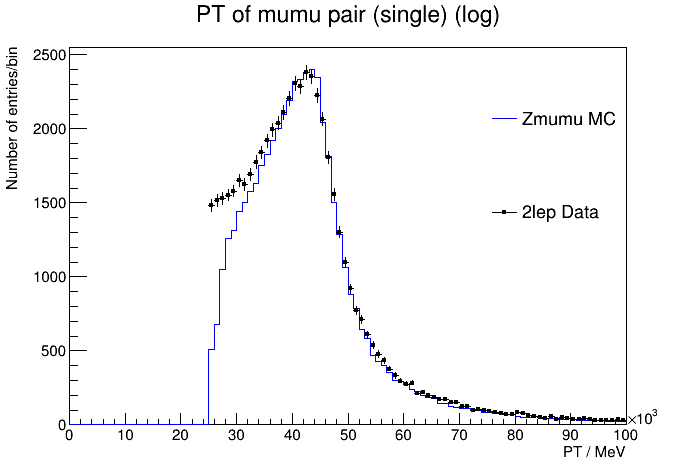
\includegraphics[width=\linewidth]{plots/27-02-2021/2-stack-Zmumu-fast_PT-single_(basic_2lep=mumu-opp-c)_27-02-21_12-00.png}
        (B)
    \end{minipage}
    \caption{(A)  (B) Transverse momentum of single muon using ATLAS and Zmumu MC data.  Cuts: (basic) muon pair of opposite charge.}
    \label{fig:2-stack-Zmumu-fast_PT-single_(basic_2lep=mumu-opp-c)_27-02-21_12-00}
\end{figure}

%%%%%%%%%%%%% 12:03 %%%%%%%%%%%%% - PT single electron (non-log)
\subsubsection*{12:03 - PT single electron}
% (B) 2-stack-fast_PT-single_(basic_2lep=ee-opp-c)_27-02-21_12-03.png
Plotting the transverse momentum of single electron of ee pair of opposite charge (standard plot).
\\
Cuts used in Fig.\ref{fig:stack-fast_PT-single_(basic_2lep=ee-opp-c)_27-02-21_12-03}
\begin{lstlisting}
lepCut = "(" + "(lep_charge[0] != lep_charge[1]) && (lep_type[0] == 11 && lep_type[1] == 11) && lep_n==2" + ")"

t.SetAlias("inv_mass_Zll","sqrt(2*lep_pt[0]*lep_pt[1]*(cosh(lep_eta[0]-lep_eta[1])-cos(lep_phi[0]-lep_phi[1])))")

t.Draw("lep_pt[0] >> h_lep_pt_total(100, 0,100e3)", weighting + "*" + lepCut)
\end{lstlisting}

\begin{figure}[h!]
    \centering
    \begin{minipage}{0.5\textwidth}
        \centering
        \includegraphics[width=\linewidth]{plots/27-02-2021/}
        (A)
    \end{minipage}\hfill
    \begin{minipage}{0.5\textwidth}
        \centering
        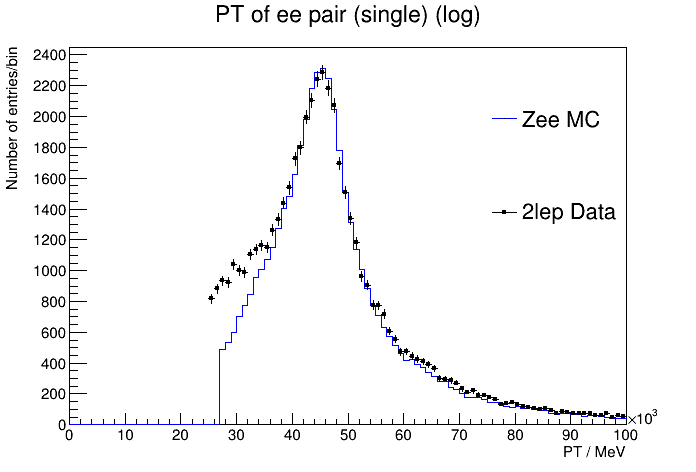
\includegraphics[width=\linewidth]{plots/27-02-2021/2-stack-fast_PT-single_(basic_2lep=ee-opp-c)_27-02-21_12-03.png}
        (B)
    \end{minipage}
    \caption{(A)  (B) Transverse momentum of single electron using both ATLAS and Zee MC data.  Cuts: (Basic) ee pair with opposite charge.}
    \label{fig:stack-fast_PT-single_(basic_2lep=ee-opp-c)_27-02-21_12-03}
\end{figure}

%%%%%%%%%%%%% 12:05 %%%%%%%%%%%%% - Invariant mass ($m_{ee}$) (log-y)
\subsubsection*{12:05 - Invariant mass ($m_{ee}$) (log-y)}
% (B) 2-Stack-Zee-fast_mll_log-y_0-200GeV_(basic_2lep=ee_opp-c)_27-02-21_12-05.png
Plotting the invariant mass of ee pair of opposite charge (log-y plot).
\\
Cuts used in Fig.\ref{fig:Stack-Zee-fast_mll_log-y_0-200GeV_(basic_2lep=ee_opp-c)_27-02-21_12-05}
\begin{lstlisting}
t.SetAlias("inv_mass_Zll","sqrt(2*lep_pt[0]*lep_pt[1]*(cosh(lep_eta[0]-lep_eta[1])-cos(lep_phi[0]-lep_phi[1])))")

# oposite charged pair of leptons (lep_n == 2)
lepCut = "(" + "(lep_charge[0] != lep_charge[1]) && lep_n==2 && lep_type[0]==11 && lep_type[1]== 11" + ")"
    
t.Draw("inv_mass_Zll >> h_inv_mass_Zll(100,0e3,200e3)", weighting + "*" + lepCut) 
\end{lstlisting}

\begin{figure}[h!]
    \centering
    \begin{minipage}{0.5\textwidth}
        \centering
        \includegraphics[width=\linewidth]{plots/27-02-2021/}
        (A)
    \end{minipage}\hfill
    \begin{minipage}{0.5\textwidth}
        \centering
        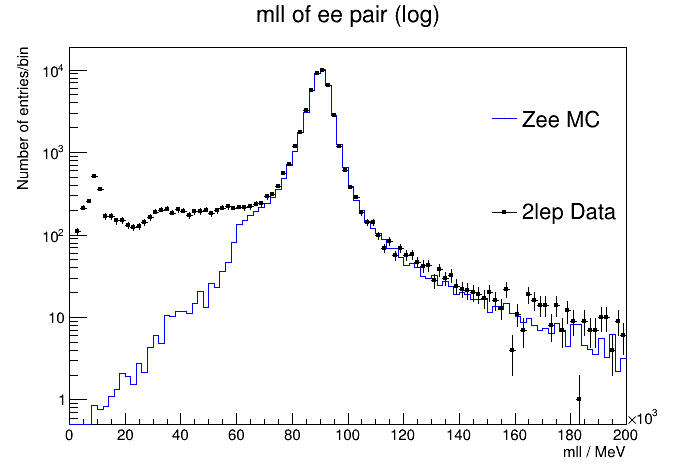
\includegraphics[width=\linewidth]{plots/27-02-2021/2-Stack-Zee-fast_mll_log-y_0-200GeV_(basic_2lep=ee_opp-c)_27-02-21_12-05.png}
        (B)
    \end{minipage}
    \caption{(A)  (B) Invariant mass of ee pair using ATLAS and Zee MC data.  Cuts: (basic) ee pair with opposite charge.}
    \label{fig:Stack-Zee-fast_mll_log-y_0-200GeV_(basic_2lep=ee_opp-c)_27-02-21_12-05}
\end{figure}

%%%%%%%%%%%%% 12:07 %%%%%%%%%%%%% - Invariant mass ($m_{\mu\mu}$) (log-y)
\subsubsection*{12:07 - Invariant mass ($m_{\mu\mu}$) (log-y)}
% (B) 2-Stack-Zmumu-fast_mll_log-y_0-200GeV_(basic_2lep=mumu_opp-c)_27-02-21_12-07.png
Plotting the invariant mass of mumu pair of opposite charge (log-y plot) with basic cuts (mumu pair with oppsite charge).
\\
Cuts used in Fig.\ref{fig:Stack-Zmumu-fast_mll_log-y_0-200GeV_(basic_2lep=mumu_opp-c)_27-02-21_12-07}
\begin{lstlisting}
t.SetAlias("inv_mass_Zll","sqrt(2*lep_pt[0]*lep_pt[1]*(cosh(lep_eta[0]-lep_eta[1])-cos(lep_phi[0]-lep_phi[1])))")

# oposite charged pair of leptons (lep_n == 2)
lepCut = "(" + "(lep_charge[0] != lep_charge[1]) && lep_n==2 && lep_type[0]==13 && lep_type[1]== 13" + ")"
    
t.Draw("inv_mass_Zll >> h_inv_mass_Zll(100,0e3,200e3)", weighting + "*" + lepCut) 
\end{lstlisting}

\begin{figure}[h!]
    \centering
    \begin{minipage}{0.5\textwidth}
        \centering
        \includegraphics[width=\linewidth]{plots/27-02-2021/}
        (A)
    \end{minipage}\hfill
    \begin{minipage}{0.5\textwidth}
        \centering
        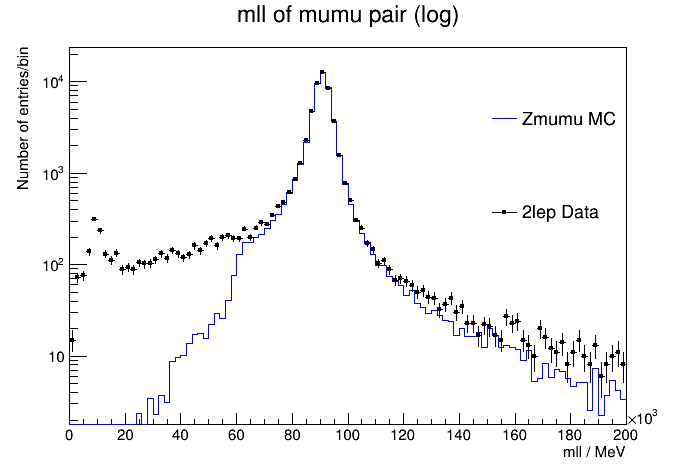
\includegraphics[width=\linewidth]{plots/27-02-2021/2-Stack-Zmumu-fast_mll_log-y_0-200GeV_(basic_2lep=mumu_opp-c)_27-02-21_12-07.png}
        (B)
    \end{minipage}
    \caption{(A)  (B) Invariant mass of mumu pair using ATLAS and Zmumu MC data.  Cuts: (basic) mumu pair with opposite charge.}
    \label{fig:Stack-Zmumu-fast_mll_log-y_0-200GeV_(basic_2lep=mumu_opp-c)_27-02-21_12-07}
\end{figure}


%%%%%%%%%%%%% 13:30 %%%%%%%%%%%%% 
\subsubsection*{13:30 - Lead BG}
Calculate the cross-section of each event ($Z \rightarrow ee$ and $Z \rightarrow \mumu$) applying various cuts on each of the variables one at a times.
\begin{itemize}
    \item ptcone30
    \item etcone20
    \item PT
    \item invariant mass
\end{itemize}
To start, however, calculate the cross section only with the basic cuts - a single lepton type pair with opposite charge.

%%%%%%%%%%%%% 13:50 %%%%%%%%%%%%% - \sigma(Z \rightarrow ee) (basic cuts) ()
\subsubsection*{13:50 - Lead BG - $\sigma(Z \rightarrow ee)$ (basic cuts)}
Calculating the cross section of $Z \rightarrow ee$ with only minimal cuts:
\begin{lstlisting}
t.SetAlias("inv_mass_Zll","sqrt(2*lep_pt[0]*lep_pt[1]*(cosh(lep_eta[0]-lep_eta[1])-cos(lep_phi[0]-lep_phi[1])))")
    
lepCut ="(" + "(lep_charge[0] != lep_charge[1]) && (lep_type[0] == 11 && lep_type[1] == 11) && lep_n==2" + ")"    
  
t.Draw("lep_n >> h_lep_n(3,-0.5,3.5)", weighting + "*" + lepCut)
\end{lstlisting}

\begin{tabular}{ | c | c | c |}
  \hline			
  var. & val. & uncert. \\
  \hline 
  
  $N^{selected}$ & 5473829 & - \\
  
  $N^{background}_{Wminus\_2lep}$ & 2.269e4 & - \\
  
  $N^{background}_{Wplus\_2lep}$ & 2.606e4 & - \\
  
  $N^{background}_{ttbar\_lep}$ & 5.56e4 & - \\
  
  $\epsilon_{num}$ & 4.737e6 & - \\
  
  $\epsilon_{den}$ & 19630128.89 & - \\
  \hline  
  $\epsilon$ &  0.24131273037199094 & - \\
  $\sigma(Z \rightarrow ee)$ &  2.2109620414181056e-09
& - \\
  \hline  
\end{tabular}

%%%%%%%%%%%%% 14:29 %%%%%%%%%%%%% - \sigma(Z \rightarrow \mu\mu) (basic cuts) ()
\subsubsection*{14:29 - $\sigma(Z \rightarrow \mu\mu)$ (basic cuts)}
Calculating the cross section of $Z \rightarrow \mu\mu$ with only minimal cuts:
\begin{lstlisting}
lepCut ="(" + "(lep_charge[0] != lep_charge[1]) && (lep_type[0] == 13 && lep_type[1] == 13) && lep_n==2" + ")"    
  
t.Draw("lep_n >> h_lep_n(3,-0.5,3.5)", weighting + "*" + lepCut)
\end{lstlisting}

\begin{tabular}{ | c | c | c |}
  \hline			
  var. & val. & uncert. \\
  \hline 
  
  $N^{selected}$ & 5669257 & - \\
  
  $N^{background}_{Wminus\_2lep}$ & 1.415e4 & - \\
  
  $N^{background}_{Wplus\_2lep}$ & 1.634e4 & - \\
  
  $N^{background}_{ttbar\_lep}$ & 4.214e4 & - \\
  
  $\epsilon_{num}$ & 5.187e6 & - \\
  
  $\epsilon_{den}$ & 19631161.45 & - \\
  \hline  
  $\epsilon$ & 0.26422277730286814 & - \\
  $\sigma(Z \rightarrow \mu\mu)$ &   2.1046771304183235e-09
& - \\
  \hline  
\end{tabular}

%%%%%%%%%%%%% 15:02 %%%%%%%%%%%%% - $\sigma(Z \rightarrow mumu)$ (etcone20 lower cut = -1.6 GeV)
\subsubsection*{15:02 - $\sigma(Z \rightarrow mumu)$ (etcone20 lower cut = -1.6 GeV)}
Calculating $\sigma(Z \rightarrow mumu)$ with the basic cuts (mumu pair with opposite charge) as well as a lower bound on the etcone20 of -1.6 GeV.  
\\
The justification of this lower bound is shown in Fig.\ref{fig:Stack-Zmumu-etcone-lower-bound-justification_27-02-21_14-52}.
\begin{figure}[h!]
    \centering
    \begin{minipage}{0.5\textwidth}
        \centering
        \includegraphics[width=\linewidth]{plots/27-02-2021/}
        (A)
    \end{minipage}\hfill
    \begin{minipage}{0.5\textwidth}
        \centering
        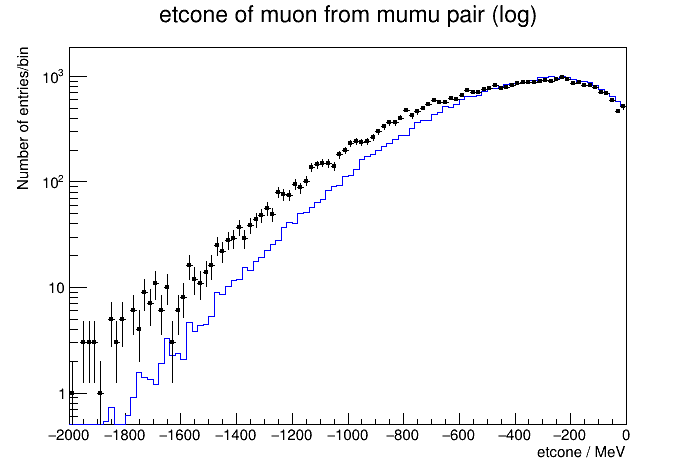
\includegraphics[width=\linewidth]{plots/27-02-2021/2-Stack-Zmumu-etcone-lower-bound-justification_27-02-21_14-52.png}
        (B)
    \end{minipage}
    \caption{(A) Lower bound justification on the etcone using the ATLAS, Zmumu MC, and MC background (B) Lower bound justification on the etcone using the ATLAS and Zmumu MC.  Cuts: (basic) pair of muons with opposite charge.}
    \label{fig:Stack-Zmumu-etcone-lower-bound-justification_27-02-21_14-52}
\end{figure}

The cuts being used to calculate the cross section:
\begin{lstlisting}
t.SetAlias("inv_mass_Zll","sqrt(2*lep_pt[0]*lep_pt[1]*(cosh(lep_eta[0]-lep_eta[1])-cos(lep_phi[0]-lep_phi[1])))")
    
lepCut ="(" + "(lep_charge[0] != lep_charge[1]) && (lep_type[0] == 13 && lep_type[1] == 13) && lep_n==2 && (lep_etcone20[0] > -1.6e3 && lep_etcone20[1] > -1.6e3)" + ")"    
  
t.Draw("lep_n >> h_lep_n(3,-0.5,3.5)", weighting + "*" + lepCut)
\end{lstlisting}

\begin{tabular}{ | c | c | c |}
  \hline			
  var. & val. & uncert. \\
  \hline 
  
  $N^{selected}$ & 5663545 & - \\
  
  $N^{background}_{Wminus\_2lep}$ & 1.414e4 & - \\
  
  $N^{background}_{Wplus\_2lep}$ & 1.632e4 & - \\
  
  $N^{background}_{ttbar\_lep}$ & 4.203e4 & - \\
  
  $\epsilon_{num}$ & 5.182e6 & - \\
  
  $\epsilon_{den}$ & 19631161.45 & - \\
  \hline  
  $\epsilon$ & 0.26396808019731305 & - \\
  $\sigma(Z \rightarrow \mu\mu)$ &   2.1046104502935312 (nb) & - \\
  \hline  
\end{tabular}


%%%%%%%%%%%%% 15:32 %%%%%%%%%%%%% - $\sigma(Z \rightarrow mumu)$ (etcone20 lower cut = -1.6 GeV) && (etcone20 upper cut = 5.25 GeV)
\subsubsection*{15:32 - $\sigma(Z \rightarrow mumu)$ cuts: ($etcone > -1.6$ GeV) && ($etcone < 5.25$ GeV)}
Calculating $\sigma(Z \rightarrow mumu)$ with the basic cuts (mumu pair with opposite charge) as well as a lower and upper bound on the etcone20 of $-1.6 GeV < etcone < 5.25 GeV$.   
\\
The justification of this upper bound is shown in Fig.\ref{fig:Stack_Zmumu-etcone-lower-bound-justification(basic)_27-02-21_15-11}

\begin{figure}[h!]
    \centering
    \begin{minipage}{0.5\textwidth}
        \centering
        \includegraphics[width=\linewidth]{plots/27-02-2021/}
        (A)
    \end{minipage}\hfill
    \begin{minipage}{0.5\textwidth}
        \centering
        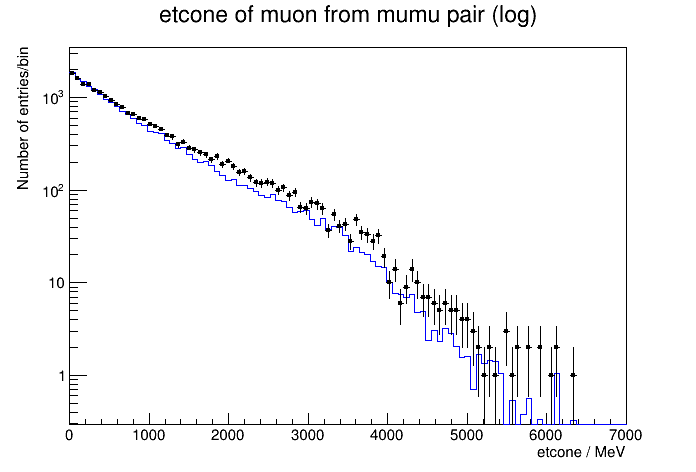
\includegraphics[width=\linewidth]{plots/27-02-2021/2-Stack_Zmumu-etcone-upper-bound-justification_(basic)_14-59.png}
        (B)
    \end{minipage}
    \caption{Upper bound justification on the etcone using the ATLAS, Zmumu MC, and MC background (B) Upper bound justification on the etcone using the ATLAS and Zmumu MC.  Cuts: (basic) pair of muons with opposite charge.}
    \label{fig:Stack_Zmumu-etcone-lower-bound-justification(basic)_27-02-21_15-11}
\end{figure}

Cuts being used to calculate the cross section of $Z \rightarrow \mu\mu$
\begin{lstlisting}
t.SetAlias("inv_mass_Zll","sqrt(2*lep_pt[0]*lep_pt[1]*(cosh(lep_eta[0]-lep_eta[1])-cos(lep_phi[0]-lep_phi[1])))")
    
lepCut ="(" + "(lep_charge[0] != lep_charge[1]) && (lep_type[0] == 13 && lep_type[1] == 13) && lep_n==2 && (lep_etcone20[0] > -1.6e3 && lep_etcone20[1] > -1.6e3) && (lep_etcone20[0] < 5.25e3 && lep_etcone20[1] < 5.25e3)" + ")"    
  
t.Draw("lep_n >> h_lep_n(3,-0.5,3.5)", weighting + "*" + lepCut)
\end{lstlisting}

\begin{tabular}{ | c | c | c |}
  \hline			
  var. & val. & uncert. \\
  \hline 
  
  $N^{selected}$ & 5657836 & - \\
  
  $N^{background}_{Wminus\_2lep}$ & 1.38e4 & - \\
  
  $N^{background}_{Wplus\_2lep}$ & 1.604e4 & - \\
  
  $N^{background}_{ttbar\_lep}$ & 4.189e4 & - \\
  
  $\epsilon_{num}$ & 5.178e6 & - \\
  
  $\epsilon_{den}$ & 19631161.45 & - \\
  \hline  
  $\epsilon$ &  0.26376432251286897 & - \\
  $\sigma(Z \rightarrow \mu\mu)$ &  2.1043718955504714 (nb) & - \\
  \hline  
\end{tabular}


%%%%%%%%%%%%% 15:47 %%%%%%%%%%%%% - $\sigma(Z \rightarrow ee)$ etcone > -2 GeV
\subsubsection*{15:47 - $\sigma(Z \rightarrow ee)$ cuts: ($etcone > -2$ GeV)}
Calculating $\sigma(Z \rightarrow ee)$ with the basic cuts (ee pair with opposite charge) as well as a lower and upper bound on the etcone20 of $-2 GeV < etcone$.   
\\
The justification of this upper bound is shown in Fig.\ref{}
% TODO: Plot the justification of the lower bound of the etcone for Z->ee

The cuts used to calculate the cross section:
\begin{lstlisting}
t.SetAlias("inv_mass_Zll","sqrt(2*lep_pt[0]*lep_pt[1]*(cosh(lep_eta[0]-lep_eta[1])-cos(lep_phi[0]-lep_phi[1])))")
    
lepCut ="(" + "(lep_charge[0] != lep_charge[1]) && (lep_type[0] == 11 && lep_type[1] == 11) && lep_n==2 && (lep_etcone20[0] > -2e3 && lep_etcone20[1] > -2e3)" + ")"    
  
t.Draw("lep_n >> h_lep_n(3,-0.5,3.5)", weighting + "*" + lepCut)
\end{lstlisting}

\begin{tabular}{ | c | c | c |}
  \hline			
  var. & val. & uncert. \\
  \hline 
  
  $N^{selected}$ & 5456608 & - \\
  
  $N^{background}_{Wminus\_2lep}$ & 2.253e4 & - \\
  
  $N^{background}_{Wplus\_2lep}$ & 2.587e4 & - \\
  
  $N^{background}_{ttbar\_lep}$ & 5.521e4 & - \\
  
  $\epsilon_{num}$ & 4.721e6 & - \\
  
  $\epsilon_{den}$ & 19630128.89 & - \\
  \hline  
  $\epsilon$ & 0.24049765676296586 & - \\
  $\sigma(Z \rightarrow ee)$ & 2.2116459465165835e-09 & - \\
  \hline  
\end{tabular}

% upper bound as well
%%%%%%%%%%%%% 16:06 %%%%%%%%%%%%% - $\sigma(Z \rightarrow ee)$ 6 GeV > etcone > -2 GeV
\subsubsection*{16:06 - $\sigma(Z \rightarrow ee)$ cuts: ($6GeV > etcone > -2$ GeV)}
Calculating $\sigma(Z \rightarrow ee)$ with the basic cuts (ee pair with opposite charge) as well as a lower and upper bound on the etcone20 of $-2 GeV < etcone < 6 GeV$.   
\\
The justification of this upper bound is shown in Fig.\ref{}
% TODO: Plot the justification of the lower bound of the etcone for Z->ee

Cuts used in calculating the cross section:
\begin{lstlisting}
t.SetAlias("inv_mass_Zll","sqrt(2*lep_pt[0]*lep_pt[1]*(cosh(lep_eta[0]-lep_eta[1])-cos(lep_phi[0]-lep_phi[1])))")
    
lepCut ="(" + "(lep_charge[0] != lep_charge[1]) && (lep_type[0] == 11 && lep_type[1] == 11) && lep_n==2 && (lep_etcone20[0] > -2e3 && lep_etcone20[1] > -2e3) && (lep_etcone20[0] < 6e3 && lep_etcone20[1] < 6e3)" + ")"    

t.Draw("lep_n >> h_lep_n(3,-0.5,3.5)", weighting + "*" + lepCut)
\end{lstlisting}

\begin{tabular}{ | c | c | c |}
  \hline			
  var. & val. & uncert. \\
  \hline 
  
  $N^{selected}$ & 5448399 & - \\
  
  $N^{background}_{Wminus\_2lep}$ & 2.224e4 & - \\
  
  $N^{background}_{Wplus\_2lep}$ & 2.559e4 & - \\
  
  $N^{background}_{ttbar\_lep}$ & 5.474e4 & - \\
  
  $\epsilon_{num}$ & 4.715e6 & - \\
  
  $\epsilon_{den}$ & 19630128.89 & - \\
  \hline  
  $\epsilon$ & 0.24019200415958145 & - \\
  $\sigma(Z \rightarrow ee)$ &  2.211494627257236 (nb) & - \\
  \hline  
\end{tabular}

%%%%%%%%%%%%% 16:14 %%%%%%%%%%%%% - $\sigma(Z \rightarrow ee) $  ptcone30 < 5800 MeV 
\subsubsection*{16:14 - $\sigma(Z \rightarrow ee)$ cuts: ($  ptcone30 < 5800 MeV $)}
Now calculating the cross section of $Z \rightarrow ee$ with basic cuts in addition to cuts of ptcone30 = ($  ptcone30 < 5800 MeV $).
\\
To start apply upper bound on the ptcone of ($ ptcone30 < 5800 MeV $).
\\
This upper bound is justified in Fig.\ref{}
% TODO: Add justification plot for the upper bound on the ptcone for Z -> ee
\\
The cuts being used to calculate the cross section:
\begin{lstlisting}
lepCut ="(" + "(lep_charge[0] != lep_charge[1]) && (lep_type[0] == 11 && lep_type[1] == 11) && lep_n==2 && (lep_ptcone30[0] < 5800 && lep_ptcone30[1] < 5800)" + ")"    
  
t.Draw("lep_n >> h_lep_n(3,-0.5,3.5)", weighting + "*" + lepCut)
\end{lstlisting}

\begin{tabular}{ | c | c | c |}
  \hline			
  var. & val. & uncert. \\
  \hline 
  
  $N^{selected}$ & 5383098 & - \\
  
  $N^{background}_{Wminus\_2lep}$ & 2.176e4 & - \\
  
  $N^{background}_{Wplus\_2lep}$ & 2.494e4 & - \\
  
  $N^{background}_{ttbar\_lep}$ & 5.271e4 & - \\
  
  $\epsilon_{num}$ & 4.705e6 & - \\
  
  $\epsilon_{den}$ & 19630128.89 & - \\
  \hline  
  $\epsilon$ & 0.23968258315394075 & - \\
  $\sigma(Z \rightarrow ee)$ & 2.190433435461428e-09 & - \\
  \hline  
\end{tabular}

%%%%%%%%%%%%% 17:08 %%%%%%%%%%%%% - $\sigma(Z \rightarrow \mu\mu) $  ptcone30 < 6500 MeV 
\subsubsection*{17:08 - $\sigma(Z \rightarrow \mu\mu)$ cuts: ($  ptcone30 < 6500 MeV $)}
Now calculating the cross section of $Z \rightarrow \mu\mu$ with basic cuts in addition to cuts of ptcone30 = ($  ptcone30 < 6500 MeV $).
\\
To start apply upper bound on the ptcone of ($ ptcone30 < 6500 MeV $).
\\
This upper bound is justified in Fig.\ref{}
% TODO: Add justification plot for the upper bound on the ptcone for Z -> \mu\mu
\\
The cuts being used to calculate the cross section:
\begin{lstlisting}
lepCut ="(" + "(lep_charge[0] != lep_charge[1]) && (lep_type[0] == 13 && lep_type[1] == 13) && lep_n==2 && (lep_ptcone30[0] < 6500 && lep_ptcone30[1] < 6500)" + ")"    
  
t.Draw("lep_n >> h_lep_n(3,-0.5,3.5)", weighting + "*" + lepCut)
\end{lstlisting}

\begin{tabular}{ | c | c | c |}
  \hline			
  var. & val. & uncert. \\
  \hline 
  
  $N^{selected}$ & - & - \\
  
  $N^{background}_{Wminus\_2lep}$ & - & - \\
  
  $N^{background}_{Wplus\_2lep}$ & - & - \\
  
  $N^{background}_{ttbar\_lep}$ & - & - \\
  
  $\epsilon_{num}$ & - & - \\
  
  $\epsilon_{den}$ & - & - \\
  \hline  
  $\epsilon$ &  - & - \\
  $\sigma(Z \rightarrow )$ & 2.102 & - \\
  \hline  
\end{tabular}

%%%%%%%%%%%%%%%%%%%%%%%%%%%%%%%%%%%%%%%%%%%%%%%%%%%%%%%%%%%%%%%%%%%%%%%%%%%%%%%%%%%%%%%%%%%%%%%%%%%%%%%%%%%%%%%%%%%%%%%%
%%%%%%%%%%%%%%%%%%%%%%%%%%%%%%%%%%%%%%%%%%%%%%%%%%%%%%%%%%%%%%%%%%%%%%%%%%%%%%%%%%%%%%%%%%%%%%%%%%%%%%%%%%%%%%%%%%%%%%%%
%%%%%%%%%%%%%%%%%%%%%%%%%%%%%%%%%%%%%%%%%%%%%%%%%%%%%%%%%%%%%%%%%%%%%%%%%%%%%%%%%%%%%%%%%%%%%%%%%%%%%%%%%%%%%%%%%%%%%%%%
%%%%%%%%%%%%%%%%%%%%%%%%%%%%%%%%%%%%%%%%%%%%%%%%%%%%%%%%%%%%%%%%%%%%%%%%%%%%%%%%%%%%%%%%%%%%%%%%%%%%%%%%%%%%%%%%%%%%%%%%
%%%%%%%%%%%%%%%%%%%%%%%%%%%%%%%%%%%%%%%%%%%%%%%%%%%%%%%%%%%%%%%%%%%%%%%%%%%%%%%%%%%%%%%%%%%%%%%%%%%%%%%%%%%%%%%%%%%%%%%%
\begin{figure}[h!]
    \centering
    \begin{minipage}{0.5\textwidth}
        \centering
        \includegraphics[width=\linewidth]{plots/27-02-2021/}
        (A)
    \end{minipage}\hfill
    \begin{minipage}{0.5\textwidth}
        \centering
        \includegraphics[width=\linewidth]{plots/27-02-2021/}
        (B)
    \end{minipage}
    \caption{(A)  (B)}
    \label{}
\end{figure}

%%%%%%%%%%%%%%%%%%%%%%%%%%%%%%%%%%%%%%%%%%%%%%%%%%%%%%%%%%%%%%%%%%%%%%%%%%%%%%%%%%%%%%%%%%%%%%%%%%%%%%%%%%%%%%%%%%%%%%%%%%%%%%%%%%%%%%%%%%%%%%%%%%%%%%%%%%%%%%%%%%%%%%%%%%%%%%%%%%%%%%%%%%%%%%%%%%%%%%%%%%%%%%%%%%%%%%%%%%%%%%%%%%%%%%%%%%%%%%%%
\begin{tabular}{ | c | c | c |}
  \hline			
  var. & val. & uncert. \\
  \hline 
  
  $N^{selected}$ & - & - \\
  
  $N^{background}_{Wminus\_2lep}$ & - & - \\
  
  $N^{background}_{Wplus\_2lep}$ & - & - \\
  
  $N^{background}_{ttbar\_lep}$ & - & - \\
  
  $\epsilon_{num}$ & - & - \\
  
  $\epsilon_{den}$ & - & - \\
  \hline  
  $\epsilon$ &  - & - \\
  $\sigma(Z \rightarrow )$ &  - & - \\
  \hline  
\end{tabular}